\documentclass[slidestop,c]{beamer}

\usepackage[utf8]{inputenc}
\usepackage[brazil]{babel}
\usepackage{ragged2e} 
\usepackage{graphicx}
\usepackage{graphics}
\usepackage{subfigure}
\usepackage{latexsym}
\usepackage{verbatim}
\usepackage{listings}
\usepackage{natbib}
\def\newblock{} %natbib workaround


%\usetheme{Warsaw}
%\usetheme{Luebeck}
\usetheme{Madrid}
\definecolor{azul}{rgb}{0.243,0.466,0.701}
\definecolor{azul2}{rgb}{0.273,0.366,0.451}
\definecolor{dgreen}{rgb}{0.273,0.206,0.421}

\setbeamercolor{frametitle}{fg=white,bg=azul2}
\setbeamercolor{subsection in head/foot}{fg=white,bg=black}

\setbeamercolor{title in head/foot}{fg=white,bg=black}

\setbeamercolor{block title}{bg=azul,fg=white}
\setbeamercolor{title}{bg=azul,fg=white}

\setbeamertemplate{navigation symbols}{} 

\useinnertheme{umbcboxes}
\setbeamercolor{umbcboxes}{bg=azul!14,fg=black}  % redefine box color!

%%%%
% Enable this lines to insert a blank slide with
% only the section name before each section 
%%%
%\AtBeginSection{
%\begin{frame}[plain]
%\begin{center}
%\structure{\Huge \textcolor{azul2}{\insertsection}}
%\end{center}
%\end{frame}
%}


\title{Presentation title}
\author[]
{
	First Author \\
	Second Author \\
    Third ...
}
\institute{Institute}
\date{Today}


\begin{document}

\setbeamertemplate{footline}
{%
\leavevmode%
\hbox{%

\begin{beamercolorbox}[wd=.9\paperwidth,ht=2.5ex,dp=1.125ex,left]{title
in head/foot}%
\usebeamerfont{author in head/foot}\hspace{.3cm}\insertshorttitle

\end{beamercolorbox}%

\begin{beamercolorbox}[wd=.1\paperwidth,ht=2.5ex,dp=1.125ex,center]{title
in head/foot}%
\usebeamerfont{author in head/foot}\insertframenumber/\inserttotalframenumber
\end{beamercolorbox}%
}%
\vskip0pt%
}

\newcommand{\be}{\begin{equation}}
\newcommand{\ee}{\end{equation}}
\newcommand{\ben}{\begin{enumerate}}
\newcommand{\een}{\end{enumerate}}
\newcommand{\beq}{\begin{eqnarray}}
\newcommand{\eeq}{\end{eqnarray}}
\newcommand{\bi}{\begin{itemize}}
\newcommand{\ei}{\end{itemize}}
\newcommand{\bde}{\begin{description}}
\newcommand{\ede}{\end{description}}
\newcommand{\treg}{®}
\newcommand{\tm}{\texttrademark}
\newcommand{\st}[1]{_{\scriptscriptstyle #1}}
\newcommand{\fmt}[1]{\frametitle{#1}}


% To create boxes with a custom title, use the following command:
% \newtheorem{teste}{Tes}



%%%%%%%%%%%%%%%%%%%%%%
% Front page
%%%%%%%%%%%%%%%%%%%%%%
\begin{frame}[plain]
  \titlepage
\end{frame}

\begin{frame}{Agenda}
  \tableofcontents
\end{frame}


%%%%%%%%%%%%%%%%%%%%%%%%%%%%%%
% Intro
%%%%%%%%%%%%%%%%%%%%%%%%%%%%%%

\section{Intro}
\subsection{Something}
%------ slide -----------------------------------------------------%
\begin{frame}[c]{Intro: Something}
    %\justifying
    \centering
    Something something something
\end{frame}

\subsection{Content}
\begin{frame}[c]{Content: text}
    \justifying
    %\centering
      Itemized this. \\
     \begin{itemize}
      \item First item;
      \item Second item;
      \item Third item;
     \end{itemize}
\end{frame}

\subsection{Image}
\begin{frame}[c]{This slide has an image}
\begin{center}
      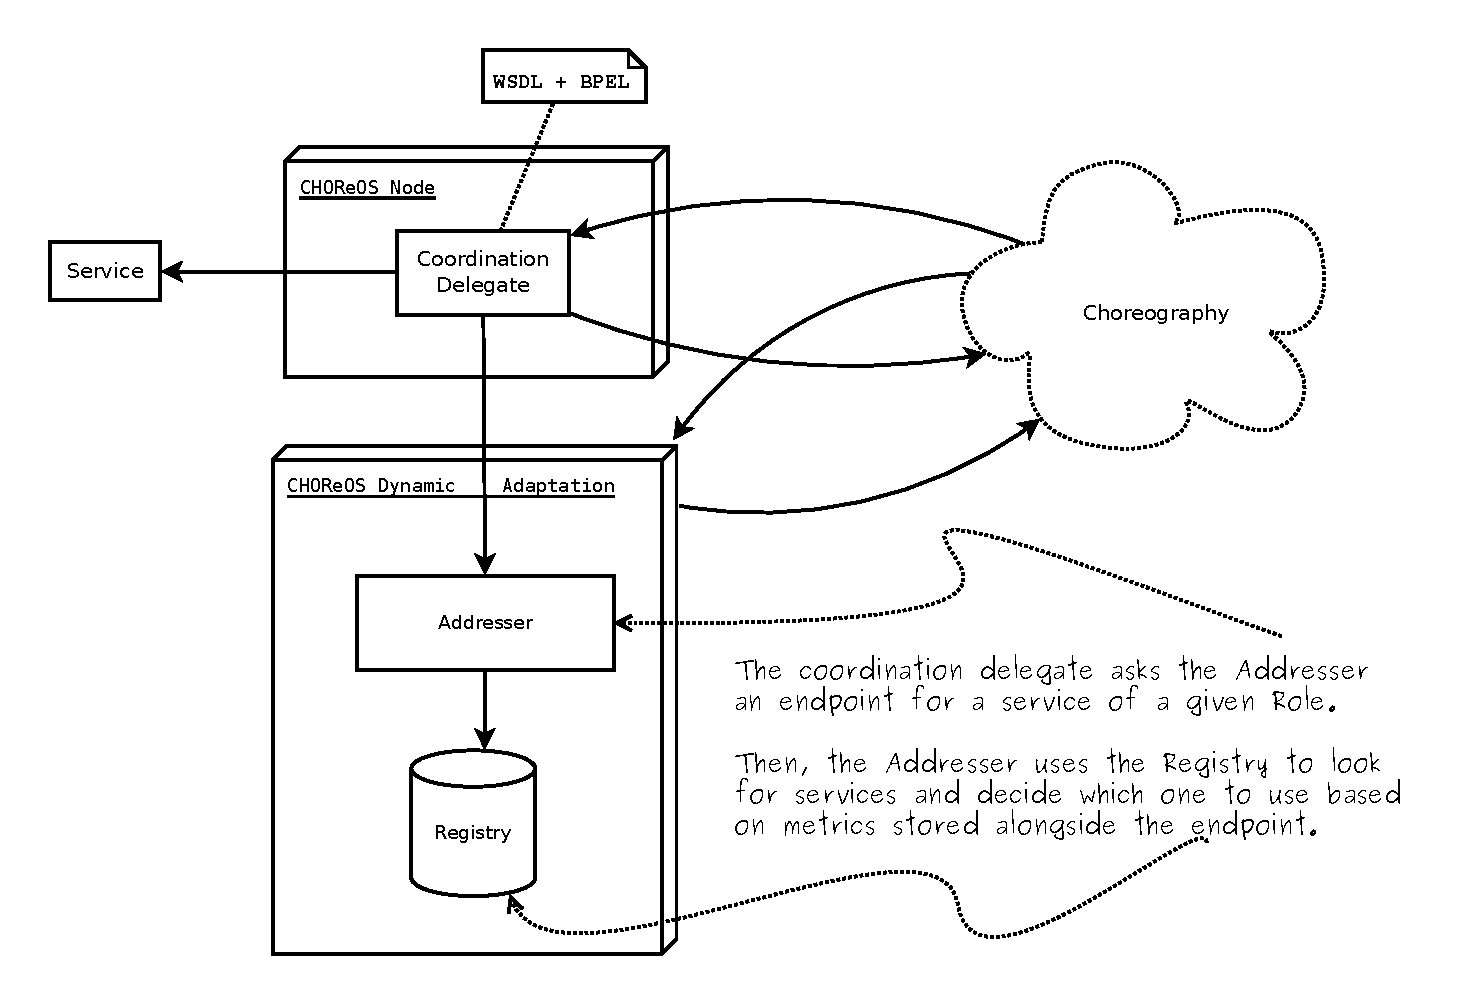
\includegraphics[width=0.8\textwidth]{figures/prototipe.pdf} \\
   \end{center}
\end{frame}

%%%%%%%%%%%%%%%%%%%%%%%%%%%%%%%%%%%%%%%%%%%%%%%%%%%%%%
\section{Blocks}
\subsection{Multiple blocks}
%%%%%%%%%%%%%%%%%%%%%%%%%%%%%%%%%%%%%%%%%%%%%%%%%%%%%%

\begin{frame}[c]{Blocks: Blocks blocks}
\begin{center}
    \begin{block}{Block 1}
        Something here.
    \end{block}
    \begin{block}{Block 2}
        other here
    \end{block}
    \begin{block}{block 3}
        and here.
    \end{block}
   \end{center}
\end{frame}


%%%%%%%%%%%%%%%%%%%%%%%
% Conclusion
\section{Future work}
%%%%%%%%%%%%%%%%%%%%%%%
\begin{frame}[c]{Futuro}
    \justifying
    %\centering
    We plan on using this template.
\end{frame}

% Final frame
\begin{frame}[plain]
\begin{center}
\structure{\Huge \textcolor{azul2}{The end. \\ Questions?}}
\end{center}
\end{frame}

\end{document}

